%% intro.tex
%% Copyright 2023 A. Grau
%
% This work may be distributed and/or modified under the conditions of the LaTeX
% Project Public License, either version 1.3 of this license or (at your option)
% any later version, with the exception that distribution of Derived Work is not
% subject to the requirements of section 6.2.
% The latest version of this license is in
%   http://www.latex-project.org/lppl.txt
% and version 1.3 or later is part of all distributions of LaTeX version
% 2005/12/01 or later.
%
% This work has the LPPL maintenance status `maintained`.
%
% The Current Maintainer of this work is A. Grau.
%
% This work consists of all the files listed in the README.md,
% and provides a copy of the original hosted on
% https://github.com/PDLT-University-of-York/UoYPhDThesis.

% The option is mandatory and points to the main file, here `thesis.tex'
\documentclass[../thesis]{subfiles}


% change title and date to appear when compiling this document on its own
\title{Single chapter: Chapter intro} \author{}
\date{(version of \today)}

% for overleaf to get the cross references, uncomment the following
% \myexternaldocument{thesis} 
% or if the file in which cross references are is known, give it direcly
% to speed up compilation, like:
% \myexternaldocument{../C-Begin/beg}

\fixsubfilexr % allow cross-ref to behave correctly

\begin{document}
% make title, tableofcontents and todolist when compiling on its own
\ifSubfilesClassLoaded{ 
	% set counter to one below the value expected to get the
	% correct number of the chapter when compiled on its own
	\setcounter{chapter}{0} 
	\maketitle \tableofcontents \listoffigures \listoftodos
	}{}

\chapter{Intro}
\todo[noline]{Write the chapters}
A quick introduction to the content of the chapter with a reference to Section~\ref{sec:in:sub} below, a cross-reference to Chapter~\ref{chap:begin} and a citation of Knuth~\cite{texbook}.

\section{A first section}
\subsection{With a subsection}\label{sec:in:sub}
\begin{figure}[h]
\centering
\caption{\textit{Research Areas by Size and Countedness} (from \href{https://xkcd.com/1991}{xkcd.com})}
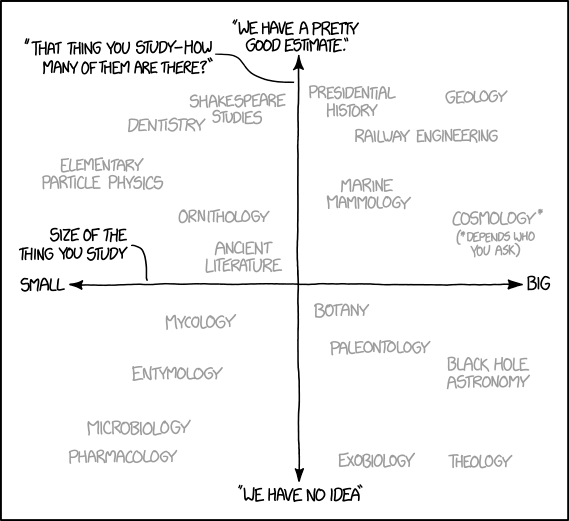
\includegraphics[draft=false,scale=.4]{xkcd1991}\\[.1em] % use draft=false to always show the image
\begin{minipage}{.68\textwidth}
\ttfamily\footnotesize 
Mathematicians give a third answer on the vertical axis, ``That question is poorly defined, but we have a sub-field devoted to every plausible version of it.''
\end{minipage}
\end{figure}
\hfill \AG

% Show bibliography page of file only if compiled on its own
\ifSubfilesClassLoaded{ 
  \printbibliography[heading=bibintoc, title=References]
  }{}
\end{document}